\chapter{Polymeren: synthese, structuur en eigenschappen}\label{ch:b2:polymer-synthesis}

Nylonkousen kwamen in 1939 in de verkoop. Ze kwamen uit een laboratorium dat zich enkele jaren
eerder had voorgenomen te begrijpen hoe kleine moleculen zich tot lange verbinden, en dat onderweg een
les had geleerd die elke chemicus de eerste keer verrast: voor een \omterm{def:b2:polymer-synthesis:polymer}{polymeer} dat gemaakt wordt door moleculen kop aan staart te koppelen,
is een rendement van 99~\% niet genoeg. Dit hoofdstuk legt uit waarom, beschrijft de twee manieren waarop ketens groeien,
en verbindt de structuur van de ketens met de eigenschappen van de materialen.
% ledger: hist:nylon-production-1939

\begin{recall}
Het schoolboek: \omterm{def:b2:polymer-synthesis:polymer}{polymeren}, \omterm{def:b2:polymer-synthesis:polymer}{monomeren} en \omterm{def:b2:polymer-synthesis:polymer}{repeterende eenheden}, additie- en condensatiepolymeren,
thermoplasten en thermoharders. Het deel van jaar~1: radicalen en homolyse, carbokationen en
carbanionen, de stationairetoestandsbenadering. \Cref{ch:b2:acyl-substitution}: esters en amiden.
\Cref{ch:b2:catalytic-cycles}: insertie in een binding metaal--koolstof.
\end{recall}

\section{Ketens en hun molaire massa's}

\begin{definition}[Polymeer]\label{def:b2:polymer-synthesis:polymer}
Een \emph{polymeer}\index{polymeer} is een stof die bestaat uit macromoleculen, die elk opgebouwd zijn door het herhaald
koppelen van kleine moleculen, de \emph{monomeren}\index{monomeer}. De \emph{repeterende eenheid}\index{repeterende eenheid}
is de kleinste groep atomen waarvan de herhaling de keten vormt; de \emph{polymerisatiegraad}\index{polymerisatiegraad}
$X$ van een keten is het aantal eenheden afkomstig van een monomeer
dat ze bevat.
\end{definition}

Een staal van een synthetisch \omterm{def:b2:polymer-synthesis:polymer}{polymeer} bestaat nooit uit identieke ketens: het is een mengsel van ketens van
verschillende lengte, en zijn molaire massa is een gemiddelde, dat afhangt van hoe de ketens geteld worden.

\begin{definition}[Gemiddelde molaire massa's]\label{def:b2:polymer-synthesis:averages}
Voor een staal met $N_i$ ketens van molaire massa $M_i$ zijn de \emph{aantalgemiddelde molaire
massa}\index{aantalgemiddelde molaire massa} en de \emph{massagemiddelde molaire massa}\index{massagemiddelde molaire massa}
gelijk aan
\begin{equation*}
\bar M_n = \frac{\sum_i N_i M_i}{\sum_i N_i}, \qquad
\bar M_w = \frac{\sum_i N_i M_i^2}{\sum_i N_i M_i} = \sum_i w_i M_i,
\end{equation*}
waarin $w_i$ de massafractie is van de ketens met massa $M_i$. De \emph{dispersiteit}\index{dispersiteit}
$\text{\DH} = \bar M_w/\bar M_n$ is minstens 1, en alleen gelijk aan 1 als alle ketens dezelfde
massa hebben. De gemiddelden $\bar X_n$ en $\bar X_w$ van de \omterm{def:b2:polymer-synthesis:polymer}{polymerisatiegraad} worden op dezelfde manier
gedefinieerd.
\end{definition}

Het aantalgemiddelde weegt elke keten één keer; het massagemiddelde weegt elke keten naar haar massa, zodat de
lange ketens zwaarder doorwegen. Dat $\text{\DH} \ge 1$ is de ongelijkheid $\left(\sum N_i M_i\right)^2 \le
\sum N_i \sum N_i M_i^2$ (Cauchy--Schwarz), met gelijkheid alleen bij gelijke $M_i$.

\begin{method}[De gemiddelden berekenen]\label{met:b2:polymer-synthesis:averages}
\begin{enumerate}
  \item Zet de gegevens om in hoeveelheden $N_i$ (of aantallen ketens) en massa's $M_i$; vanuit massafracties is
        $N_i \propto w_i/M_i$.
  \item $\bar M_n = \sum N_i M_i / \sum N_i$; of, gelijkwaardig, $1/\bar M_n = \sum w_i/M_i$.
  \item $\bar M_w = \sum w_i M_i$.
  \item $\text{\DH} = \bar M_w/\bar M_n$; controleer dat $\bar M_w \ge \bar M_n$.
\end{enumerate}
\end{method}

\section{Stapgroei en ketengroei}

\begin{definition}[Stapgroei en ketengroei]\label{def:b2:polymer-synthesis:step-chain}
Bij een \emph{stapgroeipolymerisatie}\index{stapgroeipolymerisatie} kunnen elke twee moleculen met
complementaire functionele groepen (\omterm{def:b2:polymer-synthesis:polymer}{monomeren}, oligomeren of lange ketens) reageren, en de ketens
worden langer door zich met elkaar te verbinden: polyesters, polyamiden. Bij een
\emph{ketengroeipolymerisatie}\index{ketengroeipolymerisatie} voegt een reactief centrum (radicaal, ion of binding
metaal--koolstof) monomeermoleculen één voor één toe aan het uiteinde van een groeiende keten: de \omterm{def:b2:polymer-synthesis:polymer}{polymeren} van alkenen.
\end{definition}

\begin{method}[Stapgroei of ketengroei?]\label{met:b2:polymer-synthesis:classify}
\begin{enumerate}
  \item Een \omterm{def:b2:polymer-synthesis:polymer}{monomeer} met twee functionele groepen die met elkaars partner reageren (zuur en alcohol,
        zuur en amine), vaak onder vrijzetting van een klein molecuul: stapgroei.
  \item Een \omterm{def:b2:polymer-synthesis:polymer}{monomeer} met een dubbele binding \ce{C=C} (of een gespannen ring) en een initiator: ketengroei.
  \item Controleer met het verloop van de reactie: bij stapgroei verdwijnt het \omterm{def:b2:polymer-synthesis:polymer}{monomeer} vroeg en verschijnen lange ketens
        pas helemaal op het einde; bij ketengroei verschijnen lange ketens vanaf het begin terwijl het \omterm{def:b2:polymer-synthesis:polymer}{monomeer}
        geleidelijk verbruikt wordt.
\end{enumerate}
\end{method}

\subsection*{Stapgroei}

Neem een gebalanceerd mengsel van \omterm{def:b2:polymer-synthesis:polymer}{monomeren} \ce{A-A} en \ce{B-B} (een diamine en een dizuur), of één enkel
\omterm{def:b2:polymer-synthesis:polymer}{monomeer} \ce{A-B}. Noem $p$ de \emph{omzettingsgraad}: de fractie van de functionele groepen van één
soort die gereageerd hebben.

\begin{theorem}[Vergelijking van Carothers]\label{thm:b2:polymer-synthesis:carothers}
Bij een \omterm{def:b2:polymer-synthesis:step-chain}{stapgroeipolymerisatie} van exact gebalanceerde bifunctionele \omterm{def:b2:polymer-synthesis:polymer}{monomeren} is de aantalgemiddelde
\omterm{def:b2:polymer-synthesis:polymer}{polymerisatiegraad}, geteld in monomeereenheden,
\begin{equation*}
\bar X_n = \frac{1}{1 - p}.
\end{equation*}
\end{theorem}

\begin{proof}
Begin met $N_0$ monomeermoleculen, die $N_0$ groepen \ce{A} en $N_0$ groepen \ce{B} dragen. Elke reactie
tussen een \ce{A} en een \ce{B} verbindt twee moleculen tot één, en verlaagt het aantal moleculen dus met
één. Na $pN_0$ reacties blijven er $N = N_0 - pN_0 = N_0(1-p)$ moleculen over, die de $N_0$ monomeereenheden
delen: $\bar X_n = N_0/N = 1/(1-p)$.
\end{proof}

\begin{corollary}[Onbalans]\label{cor:b2:polymer-synthesis:imbalance}
Als de groepen niet gebalanceerd zijn, met $r = N_{\ce{A}}/N_{\ce{B}} \le 1$ en $p$ de omzettingsgraad van
de minderheidsgroepen \ce{A}, dan is
\begin{equation*}
\bar X_n = \frac{1 + r}{1 + r - 2rp}, \qquad \text{hoogstens } \frac{1+r}{1-r} \text{ als } p = 1.
\end{equation*}
\end{corollary}

\begin{proof}
Bij het begin zijn er $(N_{\ce{A}} + N_{\ce{B}})/2$ bifunctionele monomeermoleculen. Elk lineair
molecuul heeft twee ketenuiteinden, elk een niet-gereageerde groep; na reactie blijven er $N_{\ce{A}}(1-p)$
groepen \ce{A} en $N_{\ce{B}} - pN_{\ce{A}}$ groepen \ce{B} over, dus $N = [N_{\ce{A}}(1-p) + N_{\ce{B}} -
pN_{\ce{A}}]/2$ moleculen. Delen, met $N_{\ce{B}} = N_{\ce{A}}/r$, geeft
$\bar X_n = (1 + 1/r)/(1 - 2p + 1/r) = (1+r)/(1 + r - 2rp)$. Met $r = 1$ is dit de vergelijking van Carothers.
\end{proof}

De vergelijking verklaart de aanhef. Bij $p = 0.99$, een ``rendement van 99~\%'' van de koppelingsreactie, is $\bar X_n =
100$; een bruikbare vezel vraagt ongeveer zoveel of meer, dus de koppeling moet verder gaan dan 99~\%, met zuivere \omterm{def:b2:polymer-synthesis:polymer}{monomeren}
in exact gelijke hoeveelheden en met verwijdering van het vrijkomende kleine molecuul (water, methanol) om het
evenwicht te blijven verschuiven. Een overmaat van 1~\% van één \omterm{def:b2:polymer-synthesis:polymer}{monomeer} beperkt $\bar X_n$ tot 201, zelfs bij volledige omzetting.

\begin{theorem}[Verdeling van Flory]\label{thm:b2:polymer-synthesis:flory}
Als bij een \omterm{def:b2:polymer-synthesis:step-chain}{stapgroeipolymerisatie} met omzettingsgraad $p$ elke groep dezelfde reactiviteit heeft, ongeacht de
lengte van haar keten, dan zijn de aantalfractie en de massafractie van ketens van $x$ eenheden
\begin{equation*}
n_x = (1-p)\,p^{\,x-1}, \qquad w_x = x(1-p)^2 p^{\,x-1},
\end{equation*}
en is $\bar X_n = 1/(1-p)$ en $\bar X_w = (1+p)/(1-p)$, zodat $\text{\DH} = 1 + p$, dicht bij 2 bij hoge
omzetting.
\end{theorem}

\begin{proof}
Volg een keten vanaf één uiteinde (een \omterm{def:b2:polymer-synthesis:polymer}{monomeer} \ce{A-B}, voor de eenvoud). Elke schakel erlangs wordt gevormd met
kans $p$, onafhankelijk van de andere. De keten heeft precies $x$ eenheden als de eerste $x-1$ schakels gevormd zijn
en de volgende niet: kans $p^{\,x-1}(1-p)$, en dat is $n_x$. Met $\sum_{x\ge1} p^{\,x-1} =
1/(1-p)$ en de afgeleiden $\sum x p^{\,x-1} = 1/(1-p)^2$ en $\sum x^2 p^{\,x-1} = (1+p)/(1-p)^3$ volgt:
$\sum n_x = 1$, $\bar X_n = \sum x n_x = 1/(1-p)$, $w_x = x n_x/\bar X_n = x(1-p)^2p^{\,x-1}$, en
$\bar X_w = \sum x w_x = (1-p)^2(1+p)/(1-p)^3 = (1+p)/(1-p)$.
\end{proof}

\begin{omfigure}
\begin{tikzpicture}
\begin{axis}[width=0.46\linewidth, height=5cm, xmin=0, xmax=400, ymin=0,
  xlabel={polymerisatiegraad $x$}, ylabel={massafractie $w_x$}, label style={font=\small},
  tick label style={font=\scriptsize}, scaled y ticks=false,
  yticklabel style={/pgf/number format/fixed, /pgf/number format/precision=3},
  legend style={font=\scriptsize, at={(0.98,0.98)}, anchor=north east}, legend cell align=left]
\addplot[omDef, thick] table[x=x, y=p95] {figdata/out/bachelor-2-polymer-distributions-a.dat};
\addplot[omThm, thick] table[x=x, y=p98] {figdata/out/bachelor-2-polymer-distributions-a.dat};
\addplot[omMeth, thick] table[x=x, y=p99] {figdata/out/bachelor-2-polymer-distributions-a.dat};
\legend{$p = 0.95$, $p = 0.98$, $p = 0.99$}
\end{axis}
\end{tikzpicture}\hfill
\begin{tikzpicture}
\begin{axis}[width=0.46\linewidth, height=5cm, xmin=0, xmax=1, ymin=0, ymax=200,
  xlabel={omzettingsgraad $p$}, ylabel={$\bar X_n$}, label style={font=\small},
  tick label style={font=\scriptsize}, xtick={0,0.2,0.4,0.6,0.8,1}]
\addplot[omDef, thick] table[x=p, y=Xn] {figdata/out/bachelor-2-polymer-distributions-b.dat};
\end{axis}
\end{tikzpicture}

{\small \omterm{def:b2:polymer-synthesis:step-chain}{Stapgroeipolymerisatie} (modellen). Links: massaverdelingen van Flory
(\cref{thm:b2:polymer-synthesis:flory}); het maximum ligt dicht bij $\bar X_n$ en de verdeling wordt breder naarmate
het naar rechts opschuift. Rechts: de vergelijking van Carothers; $\bar X_n$ blijft klein tot $p$ heel dicht bij 1 ligt.}
% figdata: bachelor-2/polymer-distributions.py parts a, b
\end{omfigure}

\subsection*{Radicalaire ketengroei}

\begin{definition}[Stappen van een ketenpolymerisatie]\label{def:b2:polymer-synthesis:chain-steps}
Een radicalaire ketenpolymerisatie verloopt in drie soorten stappen. Bij de \emph{initiatie}\index{initiatie} valt een
\emph{radicaalinitiator}\index{radicaalinitiator} (een molecuul met een zwakke binding, zoals een peroxide of een
azoverbinding) bij verhitten uiteen in radicalen, waarvan er één aan een \omterm{def:b2:polymer-synthesis:polymer}{monomeer} addeert. Bij de
\emph{propagatie}\index{propagatie} addeert het radicaal aan het ketenuiteinde een monomeermolecuul en blijft het
een radicaal. Bij de \emph{terminatie}\index{terminatie} vernietigen twee radicalen elkaar, door combinatie
(ze binden aan elkaar) of disproportionering (het ene neemt een waterstofatoom van het andere over).
\end{definition}

\begin{omfigure}
\begin{align*}
&\text{initiatie:} && \mathrm{I{-}I} \longrightarrow 2\,\mathrm{I^{\bullet}}, \qquad
\mathrm{I^{\bullet} + CH_2{=}CHPh \longrightarrow I{-}CH_2{-}\dot{C}HPh} \\
&\text{propagatie:} && {\sim}\mathrm{CH_2{-}\dot{C}HPh + CH_2{=}CHPh \longrightarrow}\;
{\sim}\mathrm{CH_2{-}CHPh{-}CH_2{-}\dot{C}HPh} \\
&\text{terminatie:} && {\sim}\mathrm{CH_2{-}\dot{C}HPh + Ph\dot{C}H{-}CH_2}{\sim} \longrightarrow
{\sim}\mathrm{CH_2{-}CHPh{-}CHPh{-}CH_2}{\sim}
\end{align*}

{\small Radicaalpolymerisatie van styreen. De initiator \ce{I-I} (dibenzoylperoxide, bijvoorbeeld)
valt uiteen in twee radicalen; elk addeert aan het \ce{CH2}-uiteinde van styreen en geeft het stabielere benzylische
radicaal; de \omterm{def:b2:polymer-synthesis:chain-steps}{propagatie} herhaalt de additie duizenden keren; twee ketenradicalen combineren en beëindigen beide
ketens. De punt markeert het ongepaarde elektron.}
\end{omfigure}

\begin{theorem}[Snelheid van radicaalpolymerisatie]\label{thm:b2:polymer-synthesis:radical-rate}
Met een initiator die ontleedt met snelheidsconstante $k_d$ en efficiëntie $f$ (de fractie radicalen die
een keten starten), propagatieconstante $k_p$ en terminatieconstante $k_t$ (terminatiesnelheid $2k_t
[\mathrm{M^\bullet}]^2$) is de stationaire polymerisatiesnelheid
\begin{equation*}
R_p = k_p [\mathrm M] \sqrt{\frac{f k_d [\mathrm I]}{k_t}}.
\end{equation*}
\end{theorem}

\begin{proof}
Zij $[\mathrm{M^\bullet}]$ de totale concentratie ketenradicalen, ongeacht hun lengte. Ze worden
gevormd met de snelheid $R_i = 2fk_d[\mathrm I]$ (twee radicalen per initiatormolecuul, waarvan een fractie $f$
een keten start) en vernietigd met de snelheid $2k_t[\mathrm{M^\bullet}]^2$; \omterm{def:b2:polymer-synthesis:chain-steps}{propagatie} zet één ketenradicaal
om in een ander en verandert hun aantal niet. De stationairetoestandsbenadering voor
$[\mathrm{M^\bullet}]$ geeft $2fk_d[\mathrm I] = 2k_t[\mathrm{M^\bullet}]^2$, dus $[\mathrm{M^\bullet}] =
\sqrt{fk_d[\mathrm I]/k_t}$. Het \omterm{def:b2:polymer-synthesis:polymer}{monomeer} wordt in hoofdzaak door \omterm{def:b2:polymer-synthesis:chain-steps}{propagatie} verbruikt, met $R_p =
k_p[\mathrm M][\mathrm{M^\bullet}]$.
\end{proof}

\begin{definition}[Kinetische ketenlengte]\label{def:b2:polymer-synthesis:chain-length}
De \emph{kinetische ketenlengte}\index{kinetische ketenlengte} $\nu$ is het gemiddelde aantal
monomeermoleculen dat geaddeerd wordt per radicaal dat een keten start: $\nu = R_p/R_i$.
\end{definition}

\begin{proposition}[Ketenlengte en initiator]\label{prop:b2:polymer-synthesis:chain-length}
In de stationaire toestand is $\nu = k_p[\mathrm M]/\bigl(2\sqrt{fk_dk_t[\mathrm I]}\bigr)$: meer initiator geeft
een snellere polymerisatie maar kortere ketens. Bij \omterm{def:b2:polymer-synthesis:chain-steps}{terminatie} door combinatie is $\bar X_n = 2\nu$; bij
disproportionering $\bar X_n = \nu$.
\end{proposition}

\begin{proof}
$\nu = R_p/R_i = k_p[\mathrm M]\sqrt{fk_d[\mathrm I]/k_t}/(2fk_d[\mathrm I]) =
k_p[\mathrm M]/\bigl(2\sqrt{fk_dk_t[\mathrm I]}\bigr)$. Elke gestarte keten addeert gemiddeld $\nu$ \omterm{def:b2:polymer-synthesis:polymer}{monomeren};
combinatie verbindt twee zulke ketens tot één molecuul, disproportionering laat er twee.
\end{proof}

\begin{definition}[Levende polymerisatie]\label{def:b2:polymer-synthesis:living}
Een \emph{levende polymerisatie}\index{levende polymerisatie} is een \omterm{def:b2:polymer-synthesis:step-chain}{ketengroeipolymerisatie} zonder
\omterm{def:b2:polymer-synthesis:chain-steps}{terminatie} of overdracht: alle ketens starten samen en blijven groeien zolang er \omterm{def:b2:polymer-synthesis:polymer}{monomeer} is, en
ze groeien weer verder wanneer er meer \omterm{def:b2:polymer-synthesis:polymer}{monomeer} toegevoegd wordt. De anionische polymerisatie van styreen, geïnitieerd door
butyllithium in een droog, aprotisch oplosmiddel, is het klassieke voorbeeld.
\end{definition}

\begin{proposition}[Smalle verdelingen]\label{prop:b2:polymer-synthesis:living}
Bij een \omterm{def:b2:polymer-synthesis:living}{levende polymerisatie} waarin alle ketens tegelijk starten, volgt de \omterm{def:b2:polymer-synthesis:polymer}{polymerisatiegraad} een
poissonverdeling, en is $\text{\DH} = 1 + \nu/(1+\nu)^2 \approx 1 + 1/\bar X_n$, waarin $\nu$ het
gemiddelde aantal \omterm{def:b2:polymer-synthesis:polymer}{monomeren} is dat per keten geaddeerd wordt.
\end{proposition}

\admitted

De verdeling is die van het aantal addities, onafhankelijke toevalsgebeurtenissen met een gemeenschappelijke snelheid, die
elke keten in dezelfde tijd ondergaat; de \omterm{def:b2:polymer-synthesis:averages}{dispersiteit} volgt uit het gemiddelde en de variantie van een poissonverdeling,
die allebei gelijk zijn aan $\nu$. Een levende keten van 100 eenheden heeft dus $\text{\DH} \approx 1.01$, tegenover bijna 2 voor
hetzelfde gemiddelde bij stapgroei.

\begin{omfigure}
\begin{tikzpicture}
\begin{axis}[width=0.72\linewidth, height=5cm, xmin=0, xmax=150, ymin=0,
  xlabel={polymerisatiegraad $x$}, ylabel={massafractie $w_x$}, label style={font=\small},
  tick label style={font=\scriptsize}, scaled y ticks=false,
  yticklabel style={/pgf/number format/fixed, /pgf/number format/precision=3},
  legend style={font=\scriptsize, at={(0.98,0.98)}, anchor=north east}, legend cell align=left]
\addplot[omThm, thick] table[x=x, y=poisson] {figdata/out/bachelor-2-polymer-distributions-c.dat};
\addplot[omDef, thick] table[x=x, y=flory] {figdata/out/bachelor-2-polymer-distributions-c.dat};
\legend{levend (Poisson), stapgroei (Flory)}
\end{axis}
\end{tikzpicture}

{\small Twee stalen met dezelfde $\bar X_n = 50$ (modellen). Levende ketens dringen samen rond 50 ($\text{\DH}
\approx 1.02$); stapgroeiketens spreiden zich uit van \omterm{def:b2:polymer-synthesis:polymer}{monomeer} tot honderden eenheden ($\text{\DH} \approx
1.98$).}
% figdata: bachelor-2/polymer-distributions.py part c
\end{omfigure}

\begin{definition}[Copolymeer]\label{def:b2:polymer-synthesis:copolymer}
Een \emph{copolymeer}\index{copolymeer} is een \omterm{def:b2:polymer-synthesis:polymer}{polymeer} dat opgebouwd is uit twee of meer verschillende \omterm{def:b2:polymer-synthesis:polymer}{monomeren}. Zijn eenheden
kunnen elkaar willekeurig opvolgen (statistisch copolymeer), afwisselend, in lange reeksen van elk
(blokcopolymeer, gemaakt door \omterm{def:b2:polymer-synthesis:living}{levende polymerisatie}), of als zijketens van het ene, geënt op een hoofdketen van het andere
(entcopolymeer).
\end{definition}

\section{Structuur van de ketens}

\begin{definition}[Tacticiteit]\label{def:b2:polymer-synthesis:tacticity}
In een vinylpolymeer \ce{-[CH2-CHR]_n-} is elk \ce{CHR}-koolstofatoom een stereocentrum. De
\emph{tacticiteit}\index{tacticiteit} beschrijft hun relatieve configuraties langs de keten, getekend als een
vlakke zigzag: in een \emph{isotactische}\index{isotactisch} keten liggen alle groepen \ce{R} aan dezelfde kant
van het vlak, in een \emph{syndiotactische}\index{syndiotactisch} keten wisselen ze af, en in een
\emph{atactische}\index{atactisch} keten staan ze willekeurig.
\end{definition}

\begin{omfigure}
\setchemfig{atom sep=1.5em}
\begin{tabular}{rl}
\small \omterm{def:b2:polymer-synthesis:tacticity}{isotactisch} & \chemfig{[:-30]-[:30](<[:90])-[:-30]-[:30](<[:90])-[:-30]-[:30](<[:90])-[:-30]-[:30](<[:90])-[:-30]-[:30](<[:90])-[:-30]} \\[2pt]
\small \omterm{def:b2:polymer-synthesis:tacticity}{syndiotactisch} & \chemfig{[:-30]-[:30](<[:90])-[:-30]-[:30](<:[:90])-[:-30]-[:30](<[:90])-[:-30]-[:30](<:[:90])-[:-30]-[:30](<[:90])-[:-30]} \\[2pt]
\small \omterm{def:b2:polymer-synthesis:tacticity}{atactisch} & \chemfig{[:-30]-[:30](<[:90])-[:-30]-[:30](<[:90])-[:-30]-[:30](<:[:90])-[:-30]-[:30](<[:90])-[:-30]-[:30](<:[:90])-[:-30]}
\end{tabular}
\par\vspace{6pt}

{\small Polypropeen getekend als zigzag in het vlak van de pagina; elke methylgroep is een wig (naar
de lezer toe) of een gearceerde wig (van de lezer af). \omterm{def:b2:polymer-synthesis:tacticity}{Isotactisch}: alle methylgroepen aan één kant; \omterm{def:b2:polymer-synthesis:tacticity}{syndiotactisch}: afwisselend;
\omterm{def:b2:polymer-synthesis:tacticity}{atactisch}: onregelmatig.}
\end{omfigure}

Regelmatige ketens kunnen zich zij aan zij schikken tot kristallijne gebieden; onregelmatige niet. \omterm{def:b2:polymer-synthesis:tacticity}{Isotactisch}
polypropeen, gemaakt met de metaalkatalysatoren van het deel van jaar~3, is gedeeltelijk kristallijn, hard en heeft een hoog
smeltpunt; \omterm{def:b2:polymer-synthesis:tacticity}{atactisch} polypropeen is een zacht, kleverig amorf materiaal. Een \omterm{def:b2:polymer-synthesis:polymer}{polymeer} is zelden volledig
kristallijn: kristallieten zitten ingebed in amorfe gebieden waar ketens verstrengeld zijn.

\begin{definition}[Thermische overgangen]\label{def:b2:polymer-synthesis:transitions}
De \emph{kristalliniteitsgraad}\index{kristalliniteitsgraad} van een \omterm{def:b2:polymer-synthesis:polymer}{polymeer} is de massafractie ervan
die in kristallijne gebieden ligt. De \emph{glasovergangstemperatuur}\index{glasovergangstemperatuur}
$T_g$ is de temperatuur waaronder de amorfe gebieden een star glas zijn, waarvan de
ketensegmenten niet kunnen bewegen, en waarboven ze rubberachtig worden; de kristallijne gebieden smelten bij een hogere
temperatuur, $T_m$.
\end{definition}

Polystyreen en poly(methylmethacrylaat) zijn amorf met een $T_g$ boven kamertemperatuur: starre,
doorzichtige glazen. Natuurrubber heeft een $T_g$ ver onder kamertemperatuur. Polyetheen, met een $T_g$ ver
onder kamertemperatuur maar sterk kristallijn, is taai en buigzaam: zijn kristallieten houden de rubberachtige
amorfe delen bij elkaar.

\begin{omfigure}
\begin{tikzpicture}[x=1cm, y=1cm]
\draw[->] (0,0) -- (8.6,0) node[below left, font=\small] {temperatuur};
\draw[->] (0,0) -- (0,4.6) node[above, font=\small] {$\log$ modulus};
\draw[omDef, very thick] (0.2,4) .. controls (1.8,3.95) and (2.4,3.9) .. (2.8,3.6)
  .. controls (3.3,3.0) and (3.4,1.9) .. (4.0,1.75) -- (6.0,1.6)
  .. controls (6.7,1.5) and (7.0,0.8) .. (7.8,0.35);
\draw[omThm, very thick, dashed] (4.0,1.75) -- (6.0,1.7) .. controls (6.6,1.68) and (7.2,1.65) .. (8.2,1.6);
\draw[densely dotted] (3.2,0) node[below, font=\small] {$T_g$} -- (3.2,4.2);
\node[font=\footnotesize, align=center] at (1.4,3.4) {glasachtig};
\node[font=\footnotesize, align=center] at (4.0,3.3) {overgang};
\node[font=\footnotesize, align=center] at (5.0,2.3) {rubberplateau};
\node[font=\footnotesize, align=center, omDef] at (7.6,1.15) {vloei};
\node[font=\footnotesize, align=center, omThm] at (7.7,2.0) {vernet};
\end{tikzpicture}
\par\vspace{4pt}

{\small Modulus (stijfheid) van een amorf \omterm{def:b2:polymer-synthesis:polymer}{polymeer} tegen de temperatuur, schematisch. Onder $T_g$ is het
materiaal een glas; doorheen de overgang daalt de modulus met ordes van grootte; op het
rubberplateau gedragen verstrengelde ketens zich als een rubber; bij hogere temperatuur vloeit een lineair \omterm{def:b2:polymer-synthesis:polymer}{polymeer} (doorgetrokken
lijn), terwijl een vernet \omterm{def:b2:polymer-synthesis:polymer}{polymeer} zijn plateau behoudt tot het ontleedt (gestreept).}
\end{omfigure}

\section{Eigenschappen en toepassingen}

\begin{definition}[Elastomeer]\label{def:b2:polymer-synthesis:elastomer}
Een \emph{elastomeer}\index{elastomeer} is een \omterm{def:b2:polymer-synthesis:polymer}{polymeer} dat boven zijn \omterm{def:b2:polymer-synthesis:transitions}{glasovergangstemperatuur} gebruikt wordt en waarvan de
ketens licht vernet zijn: het kan tot verscheidene keren zijn lengte uitgerekt worden en neemt zijn
vorm weer aan wanneer het losgelaten wordt.
\end{definition}

De vier grote klassen van polymeermaterialen volgen uit structuur en overgangen. Thermoplasten,
lineair of vertakt, glasachtig of semikristallijn bij kamertemperatuur, worden zacht bij verhitten en kunnen
telkens opnieuw gevormd worden: polyetheen, polypropeen, polystyreen, PET. \omterm{def:b2:polymer-synthesis:elastomer}{Elastomeren} zijn licht
vernette ketens boven hun $T_g$: gevulkaniseerd rubber, waarin zwavelbruggen de ketens verbinden.
Vezels zijn ketens die door verstrekken gericht zijn, met sterke interacties ertussen: de waterstofbruggen tussen
amidegroepen in nylon. Thermoharders zijn dicht vernette netwerken die tijdens het vormen ontstaan: epoxy- en
fenol-formaldehydeharsen, die niet opnieuw gesmolten kunnen worden. Alleen thermoplasten worden door smelten gerecycleerd; het
schoolboek gaf de omvang van het probleem.

\begin{omfigure}
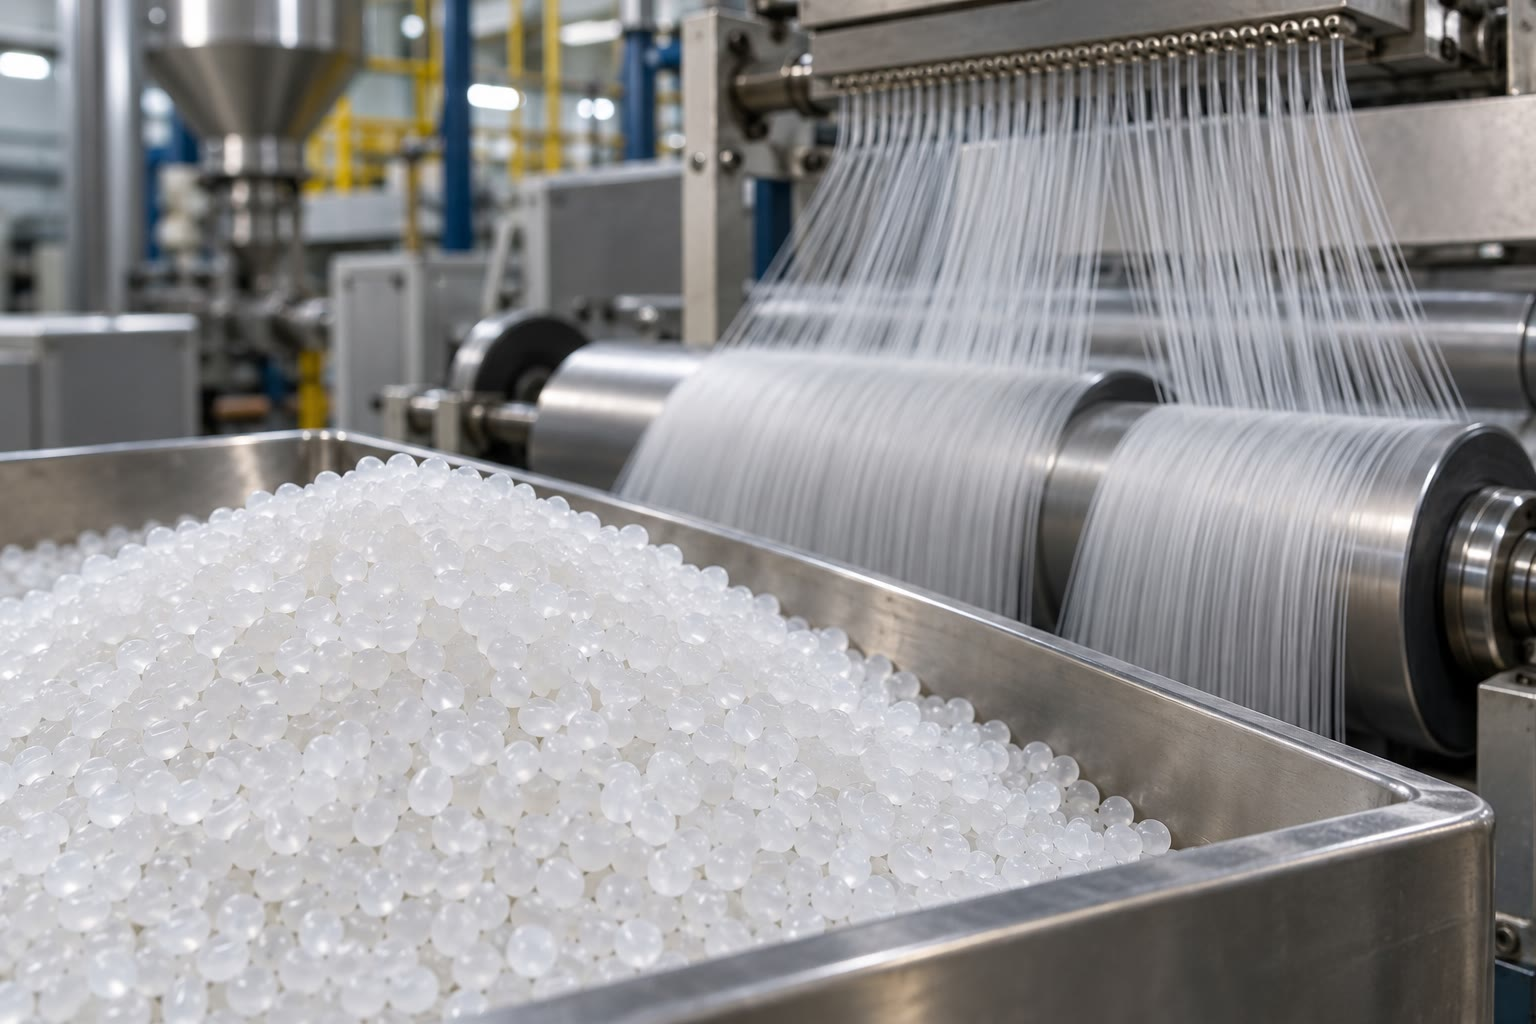
\includegraphics[width=0.58\linewidth]{images/book3/ai/b2-29-pellets.jpg}

{\small Polymeerkorrels in een fabriek, de vorm waarin thermoplasten verkocht worden, en vezels die erachter
uit een spindop op draaiende rollen getrokken worden (illustratie).}
\end{omfigure}

\begin{history}[Een rendement van 99~\% is niet genoeg]
\begin{minipage}[t]{0.2\linewidth}
\vspace{0pt}
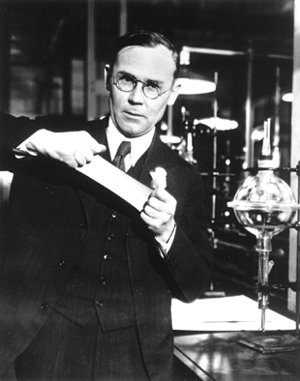
\includegraphics[width=\linewidth]{images/book3/carothers.jpg}
\end{minipage}\hfill
\begin{minipage}[t]{0.76\linewidth}
\vspace{0pt}
Wallace Carothers, een jonge universitaire docent die door een industrieel laboratorium aangeworven was voor
fundamenteel onderzoek, bouwde lange moleculen met welbekende reacties, en zijn resultaten ondersteunden sterk
het toen nog betwiste idee dat \omterm{def:b2:polymer-synthesis:polymer}{polymeren} gewone moleculen zijn, alleen heel lang. Zijn team
maakte polyesters, en vanaf 1934 polyamiden; de vergelijking die zijn naam draagt, verklaart waarom alleen
extreme omzettingen vezels gaven. Nylon ging in 1939 in productie. (Foto: onbekende
fotograaf, publiek domein; Wikimedia Commons.)
% ledger: hist:polyamides-1934, hist:nylon-production-1939
\end{minipage}
\end{history}

\begin{safety}{\ghs[5mm]{GHS01}\,\ghs[5mm]{GHS02}\,\ghs[5mm]{GHS05}\,\ghs[5mm]{GHS07}\,\ghs[5mm]{GHS08}\,\ghs[5mm]{GHS09}}
Styreen is ontvlambaar en schadelijk voor de gezondheid. Dibenzoylperoxide is in droge toestand een explosieve oxidator en wordt
vochtig en koel bewaard. Hexaan-1,6-diamine en hexaandizuur zijn corrosief voor de ogen.
% ledger: ghs:styrene, ghs:BPO, ghs:hexanediamine, ghs:adipic-acid
\end{safety}

\section{Oefeningen}

\begin{exercise}[$\star$]\label{exo:b2:polymer-synthesis:1}
Teken de \omterm{def:b2:polymer-synthesis:polymer}{repeterende eenheden} van polyetheen, polypropeen, poly(vinylchloride), polystyreen en nylon-6,6.
\end{exercise}

\begin{exercise}[$\star$]\label{exo:b2:polymer-synthesis:2}
Stapgroei of ketengroei: PET uit ethaan-1,2-diol en benzeen-1,4-dicarbonzuur; polystyreen;
nylon-6,6; poly(methylmethacrylaat); poly(melkzuur) uit 2-hydroxypropaanzuur?
\end{exercise}

\begin{exercise}[$\star$]\label{exo:b2:polymer-synthesis:3}
Een polystyreen heeft $\bar X_n = 1000$. Bereken $\bar M_n$, met verwaarlozing van de eindgroepen.
\end{exercise}

\begin{exercise}[$\star$]\label{exo:b2:polymer-synthesis:4}
Een polypropeenketen, getekend als vlakke zigzag, heeft haar methylgroepen aan de kant van de lezer, dan
van de lezer af, dan naar de lezer toe, dan weer af, enzovoort. Geef haar \omterm{def:b2:polymer-synthesis:tacticity}{tacticiteit}. Zou ze kunnen kristalliseren?
\end{exercise}

\begin{exercise}[$\star\star$]\label{exo:b2:polymer-synthesis:5}
Een staal is een mengsel van gelijke massa's van twee fracties, met molaire massa's \qty{10}{kg/mol} en
\qty{100}{kg/mol}. Bereken $\bar M_n$, $\bar M_w$ en de \omterm{def:b2:polymer-synthesis:averages}{dispersiteit}.
\end{exercise}

\begin{exercise}[$\star\star$]\label{exo:b2:polymer-synthesis:6}
Bereken $\bar X_n$ voor een gebalanceerde \omterm{def:b2:polymer-synthesis:step-chain}{stapgroeipolymerisatie} bij $p = 0.98$ en $p = 0.995$.
\end{exercise}

\begin{exercise}[$\star\star$]\label{exo:b2:polymer-synthesis:7}
Een dizuur en een diamine worden gemengd met een overmaat van 1~\% (in mol) diamine. Wat is de grootste
$\bar X_n$ die bereikt kan worden?
\end{exercise}

\begin{exercise}[$\star\star$]\label{exo:b2:polymer-synthesis:8}
Bij een radicaalpolymerisatie wordt de initiatorconcentratie verdubbeld. Met welke factor veranderen de
polymerisatiesnelheid en de \omterm{def:b2:polymer-synthesis:chain-length}{kinetische ketenlengte}?
\end{exercise}

\begin{exercise}[$\star\star$]\label{exo:b2:polymer-synthesis:9}
Poly(vinylchloride) is star; tuinslangen die ervan gemaakt zijn, zijn buigzaam omdat ze een weekmaker bevatten,
een klein molecuul dat tussen de ketens gemengd is. Leg uit met de glasovergang.
\end{exercise}

\begin{exercise}[$\star\star\star$]\label{exo:b2:polymer-synthesis:10}
Toon aan dat de massaverdeling van Flory $w_x = x(1-p)^2p^{\,x-1}$, beschouwd als functie van een continue
$x$, maximaal is bij $x = -1/\ln p$, en dat dit dicht bij $\bar X_n$ ligt wanneer $p$ dicht bij 1 ligt.
\end{exercise}

\begin{exercise}[$\star\star\star$]\label{exo:b2:polymer-synthesis:11}
PET wordt in twee fasen gemaakt: dimethylbenzeen-1,4-dicarboxylaat geeft met een overmaat ethaan-1,2-diol
bis(2-hydroxyethyl)benzeen-1,4-dicarboxylaat en methanol; daarna wordt die diester onder vacuüm verhit
en polymeriseert hij, waarbij ethaan-1,2-diol vrijkomt. Schrijf beide fasen op en leg uit hoe de tweede fase
het stoichiometrieprobleem van de vergelijking van Carothers oplost.
\end{exercise}

\begin{exercise}[$\star\star\star$]\label{exo:b2:polymer-synthesis:12}
Bij een radicalaire copolymerisatie van de \omterm{def:b2:polymer-synthesis:polymer}{monomeren} 1 en 2 wordt de momentane samenstelling van het \omterm{def:b2:polymer-synthesis:copolymer}{copolymeer}
gegeven door $\dfrac{\mathrm d[\mathrm M_1]}{\mathrm d[\mathrm M_2]} = \dfrac{[\mathrm M_1](r_1[\mathrm M_1]
+ [\mathrm M_2])}{[\mathrm M_2]([\mathrm M_1] + r_2[\mathrm M_2])}$, waarin $r_1$ en $r_2$ de
reactiviteitsverhoudingen zijn (gegevens voor de oefening: $r_1 = 2.0$, $r_2 = 0.5$). Bereken de verhouding van de eenheden in het
\omterm{def:b2:polymer-synthesis:copolymer}{copolymeer} dat gevormd wordt uit een equimolaire voeding. Wat gebeurt er als $r_1 = r_2 = 0$?
\end{exercise}

\section{Probleem: nylon-6,6 per kilogram}

\begin{problem}[{Weekendprobleem --- de monomeren en het nylonzout, de vergelijking van Carothers, een
opzettelijke onbalans, de verdeling van Flory en het vrijkomende water}]
\label{pb:b2:polymer-synthesis:1}
Nylon-6,6 wordt gemaakt uit hexaan-1,6-diamine en hexaandizuur. Eindgroepen worden overal verwaarloosd.
Molaire massa's (\unit{g/mol}): C 12.011, H 1.008, N 14.007, O 15.999.
% ledger: aw:C, aw:H, aw:N, aw:O, ghs:hexanediamine, ghs:adipic-acid

\medskip
\noindent\textbf{Deel I --- \omterm{def:b2:polymer-synthesis:polymer}{Monomeren} en \omterm{def:b2:polymer-synthesis:polymer}{repeterende eenheid}.}
\begin{enumerate}
  \item Schrijf de formules van de twee \omterm{def:b2:polymer-synthesis:polymer}{monomeren} op.
  \item Schrijf de vergelijking op van de vorming van één amidebinding.
  \item De \omterm{def:b2:polymer-synthesis:polymer}{monomeren} worden eerst gecombineerd tot een zout 1\,:\,1, dat uit oplossing gekristalliseerd wordt. Waarom?
  \item Geef de \omterm{def:b2:polymer-synthesis:polymer}{repeterende eenheid} van nylon-6,6, haar formule en haar molaire massa.
  \item Wat is de gemiddelde molaire massa $M_0$ van een eenheid in de keten die van een \omterm{def:b2:polymer-synthesis:polymer}{monomeer} afkomstig is?
  \item Wat tellen de twee getallen in de naam ``6,6''?
\end{enumerate}

\medskip
\noindent\textbf{Deel II --- De vergelijking van Carothers.}
\begin{enumerate}[resume]
  \item Bereken $\bar X_n$ en $\bar M_n$ bij $p = 0.98$.
  \item Hetzelfde bij $p = 0.99$.
  \item Verklaar de opmerking ``een rendement van 99~\% is niet genoeg''.
  \item Welke omzettingsgraad geeft $\bar M_n = \qty{10}{kg/mol}$?
  \item Hoe wordt de omzettingsgraad in de praktijk zo hoog opgedreven?
  \item Waarom moeten de \omterm{def:b2:polymer-synthesis:polymer}{monomeren} zeer zuiver zijn?
\end{enumerate}

\medskip
\noindent\textbf{Deel III --- Een opzettelijke onbalans.}
\begin{enumerate}[resume]
  \item Het diamine wordt in een molaire overmaat van 1~\% gebruikt. Bereken $r$.
  \item Bereken de grootste $\bar X_n$ en $\bar M_n$ die dan bereikt kunnen worden.
  \item Bereken $\bar X_n$ bij $p = 0.99$ met deze onbalans.
  \item Welke groepen sluiten de ketens af op het einde van de reactie?
  \item Soms wordt een beetje ethaanzuur toegevoegd. Wat doet dat met de ketens?
  \item Waarom zou een fabrikant de ketenlengte opzettelijk beperken?
\end{enumerate}

\medskip
\noindent\textbf{Deel IV --- Verdeling en massabalans.}
\begin{enumerate}[resume]
  \item Geef de \omterm{def:b2:polymer-synthesis:averages}{dispersiteit} voor een gebalanceerd mengsel bij $p = 0.99$.
  \item Bereken $\bar M_w$ bij $p = 0.99$.
  \item Welke fractie van de moleculen, en welke fractie van de massa, is bij $p = 0.99$ nog
        niet-gereageerd \omterm{def:b2:polymer-synthesis:polymer}{monomeer}?
  \item Bij welke ketenlengte is de massaverdeling het grootst?
  \item Bereken de massa water die per kilogram nylon-6,6 vrijkomt.
  \item Waarom vraagt smeltspinnen een $\bar M_n$ binnen een bepaald venster?
  \item Geef de omzettingsgraad die voor een gebalanceerd mengsel $\bar M_n = \qty{20}{kg/mol}$ geeft.
\end{enumerate}
\end{problem}
